We call {\em focus-inversive} (or simply {\em inversive}) the family of triangles which are the inversive image of billiard N-periodics with respect to a circle centered on a focus. The $N=3$ case is shown in \cref{fig:08-n3-finv}.

Note that since the inversive image of an ellipse with respect to a focus is a loopless Pascal's Limaçon, see \cite{mw}, the focus-inversive is inscribed in such a curve ans is therefore not Ponceletian. Indeed, the caustic is also non-elliptic. As shown in \cref{fig:08-n3-caustics}, a continuously increasing billiard aspect ratio will transition the caustic from (i) a regular curve, to (ii) one with a self-intersection and two cusps, to (iii) a non-compact curve with two infinite branches.

\begin{figure}
    \centering
    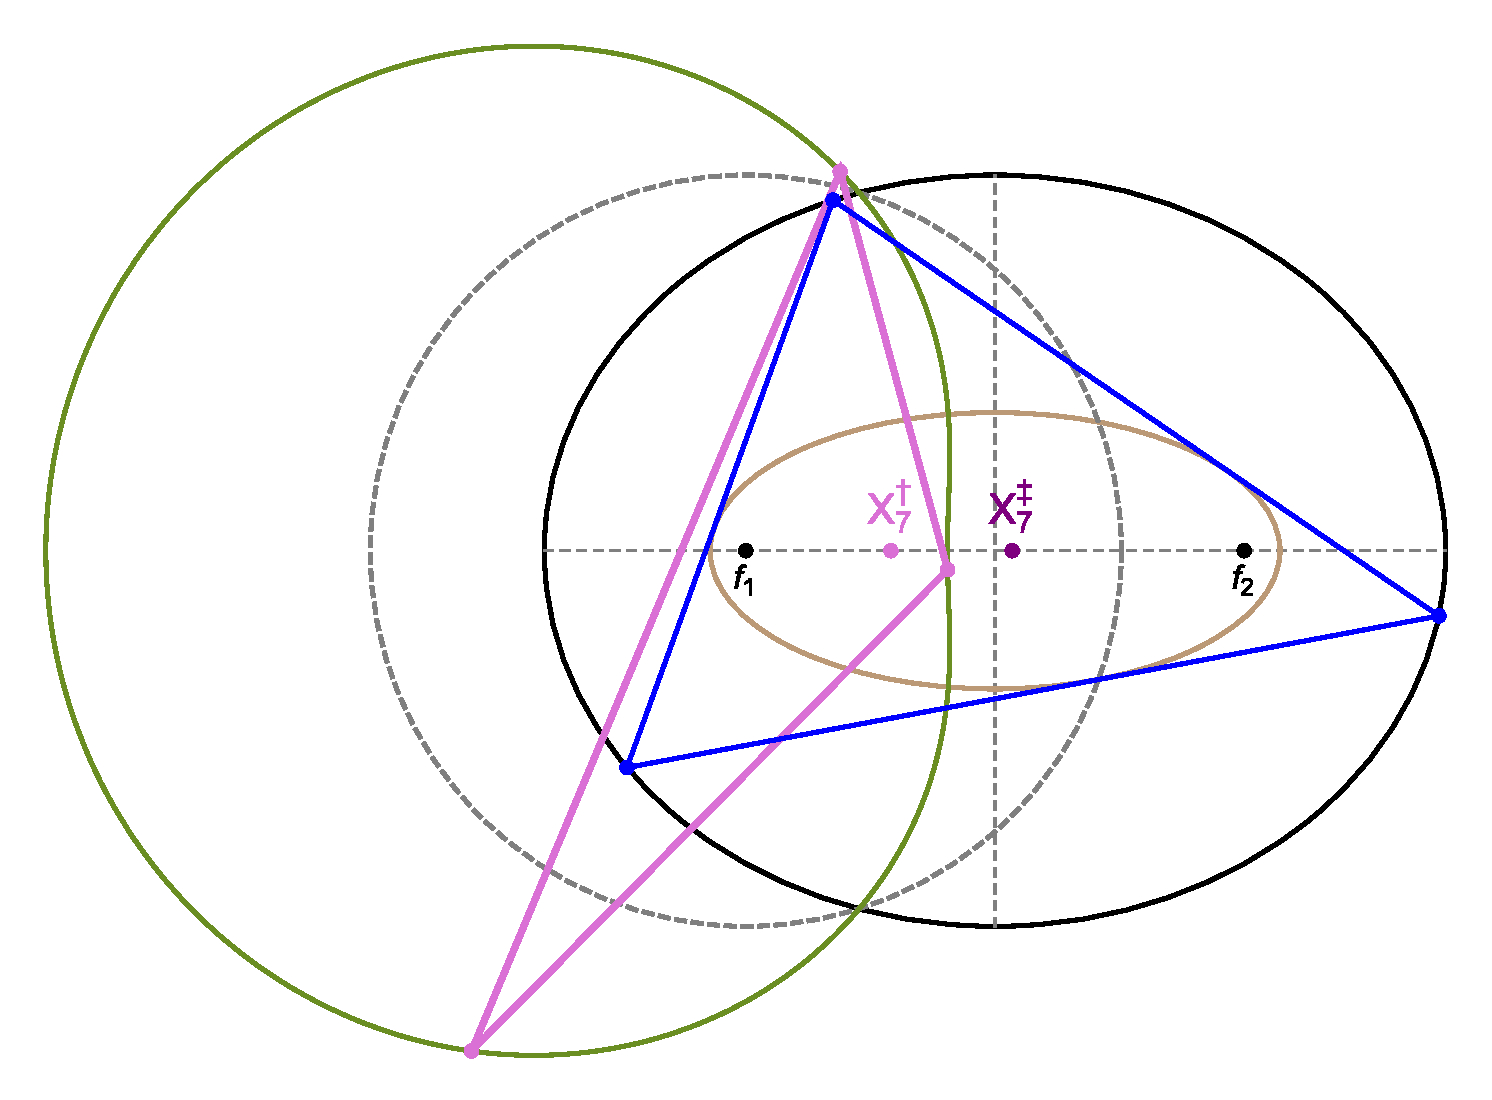
\includegraphics[width=.8\textwidth]{pics_08_010_n3_finv.eps}
    \caption{The $N=3$ focus-inversive family (pink), i.e., the inversive image of billiard 3-periodics (blue) with respect to a focused-centered circle $\Cm$ (dashed gray). Focus-inversives are inscribed in a loopless Pascal's Limaçon (olive green). Both perimeter and sum of cosines are invariant. The Gergonne point $X_7^\dagger$ is stationary. Also shown is $X_7^\ddagger$, the inversive image of $X_7^\dagger$ with respect to $\Cm$, inquired about in \cref{exe:08-x7-ddagger}. \href{https://bit.ly/3i19g6Q}{Live}}
    \label{fig:08-n3-finv}
\end{figure}

\begin{figure}
    \centering
    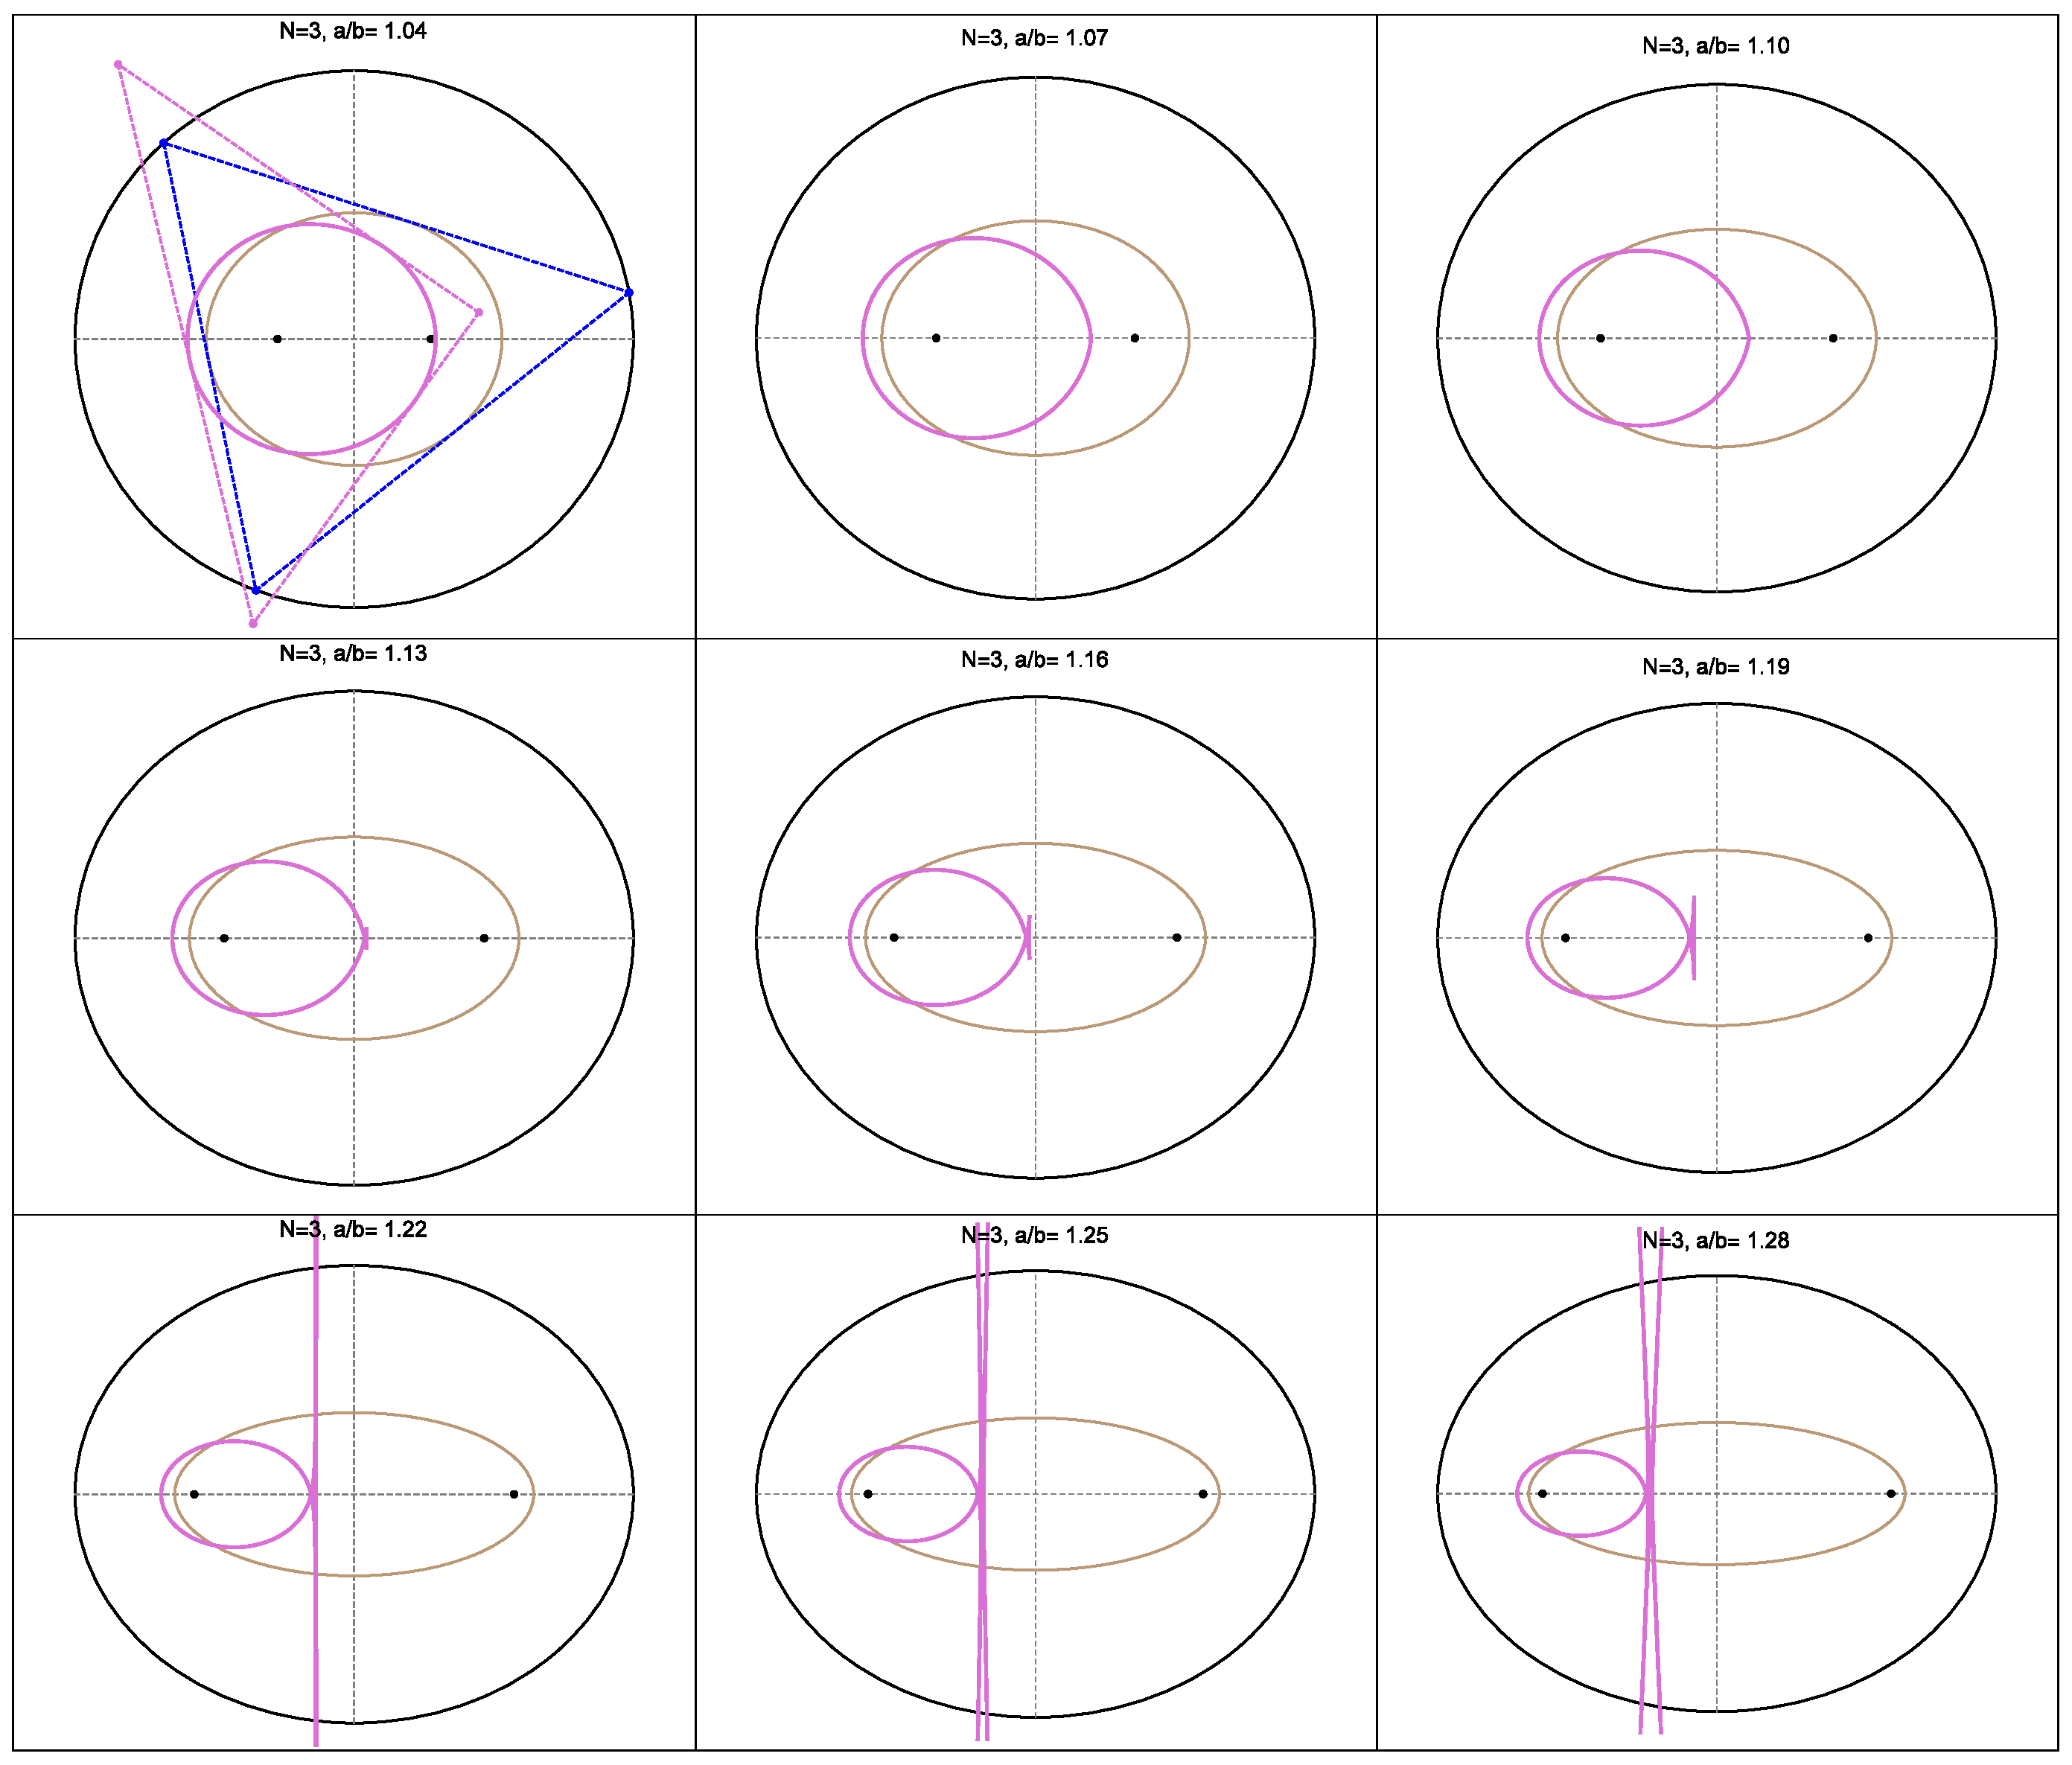
\includegraphics[width=\textwidth]{pics_08_020_n3_caustic.eps}
    \caption{Non-conic caustic (pink) to the focus-inversive family (pink). A billiard 3-periodic (dashed blue) and the corresponding focus-inversive triangle are shown at the top-left picture only. The billiard caustic is shown on every frame (brown). From left-to-right, top-to-bottom, $a/b$ is increased in small steps. Over this range, the caustic transitions from (i) a regular curve, to (ii) a curve with one self-intersection and two cusps, to (iii) a non-compact curve.  \href{https://bit.ly/374jbBl}{Live}}
    \label{fig:08-n3-caustics}
\end{figure}

\section{A stationary point}

Recall in the confocal family the Mittenpunkt $X_9$ is stationary. Henceforth we shall append a $\dagger$ to all quantities referring to the focus-inversive family. Let $a,b$ denote the semi-axes of the pre-inversion billiard which we assume to be centered on $[0,0]$ and be axis-parallel to $x$, and $y$ respectively. Let $\rho$ denote the radius of $f_1=[-c,0]$, the (left) focus-centered inversion circle, $c^2=a^2-b^2$. Interestingly:

\begin{proposition}
The Gergonne point $X_7^\dagger$ of focus-inversives is stationary on the major axis of the pre-image confocal pair. Its coordinates are given by:
\[ X_7^\dagger=\left[c\left(1-\frac{\rho^2}{\delta+c^2}\right),0\right]\]
where as before: $\delta^2=a^4-(a b)^2+b^4$.
\label{prop:08-gergonne}
\end{proposition} 

\section{Billiard-like invariants}

The following two surprising invariants -- constant perimeter and sum of cosines -- are analogues to those displayed by billiard 3-periodics. Interestingly they are not consequences of elementary principles or transformations. 

\begin{proposition}
The perimeter $L^\dagger$ of focus-inversives is invariant and given by: 
\[L^\dagger=\rho^2 \frac {\sqrt { \left( 8\,{a}^{4}+4\,{a}^{2}{b}^{2}+2\,{b}^{4}
 \right) \delta+8\,{a}^{6}+3\,{a}^{2}{b}^{4}+2\,{b}^{6}}}{{a}^{2}{b}^{
2}}\]
\label{prop:08-inv-perimeter}
\end{proposition}

Let $\theta_i^\dagger$ denote angles internal to focus-inversives. 

\begin{proposition}
The sum of internal angle cosines of focus-inversives is invariant and given by: 
\[
\sum\cos{\theta_{1,i}^\dagger}=\frac{\delta (a^2+c^2-\delta)}{a^2c^2} \]
\label{prop:08-inv-cos-sum}
\end{proposition}

\section{The rotating billiard table}

Recall that in \cref{fig:02-circumbilliard} we introduced the concept of the {\em circumbilliard}: given a triangle $T$, this is the $X_9$-centered circumellipse of which $T$ is a billiard 3-periodic (circumellipse normals are angular bisectors). Let  $\mathcal{C}^\dagger$ denote the (moving) circumbilliard ($X_9^\dagger$-centered circumellipse) of focus-inversives. Indeed, and referring to \cref{fig:08-n3-moving-billiard-table}, focus-inversives are billiard 3-periodics of a rigidly-moving virtual elliptic billiard (see \cref{exe:08-moving-billiard-table}):

\begin{proposition}
Over focus-inversives, the semi-axes $a^\dagger,b^\dagger$ of $\mathcal{C}^\dagger$ are invariant and given by:

\begin{align*}
    a^\dagger&= \rho\,k_1
\sqrt {k_2\left(\delta+a\,c\right)}\\
    b^\dagger&= \rho\,k_1
\sqrt {k_2\left(\delta-a\,c\right) }\\
 \mbox{where:}&\\
k_1&=\frac{c \sqrt{2}}{k_3}\sqrt { \left( 8\,{a}^{4}+4\,{a}^{2}{b}^{2}+2\,{b}^{4}
 \right) \delta+8\,{a}^{6}+3\,{a}^{2}{b}^{4}+2\,{b}^{6}}\\
 k_2&=2 a^2-b^2-\delta\\
 %\sqrt{ \left( -4\,{a}^{2}+2\,{b}^{2} \right) \delta+5\,{a}^{4}-5\,{a}^{2}{b}^{2}+2\,{b}^{4}}\\
k_3&=2a  {b}^{2} \left(  \left( 2\,{a}^{2}-{b}^{2} \right) \delta+2
\,{a}^{4}-2\,{a}^{2}{b}^{2}-{b}^{4}\right)
\end{align*}
\end{proposition}

\begin{figure}
    \centering
    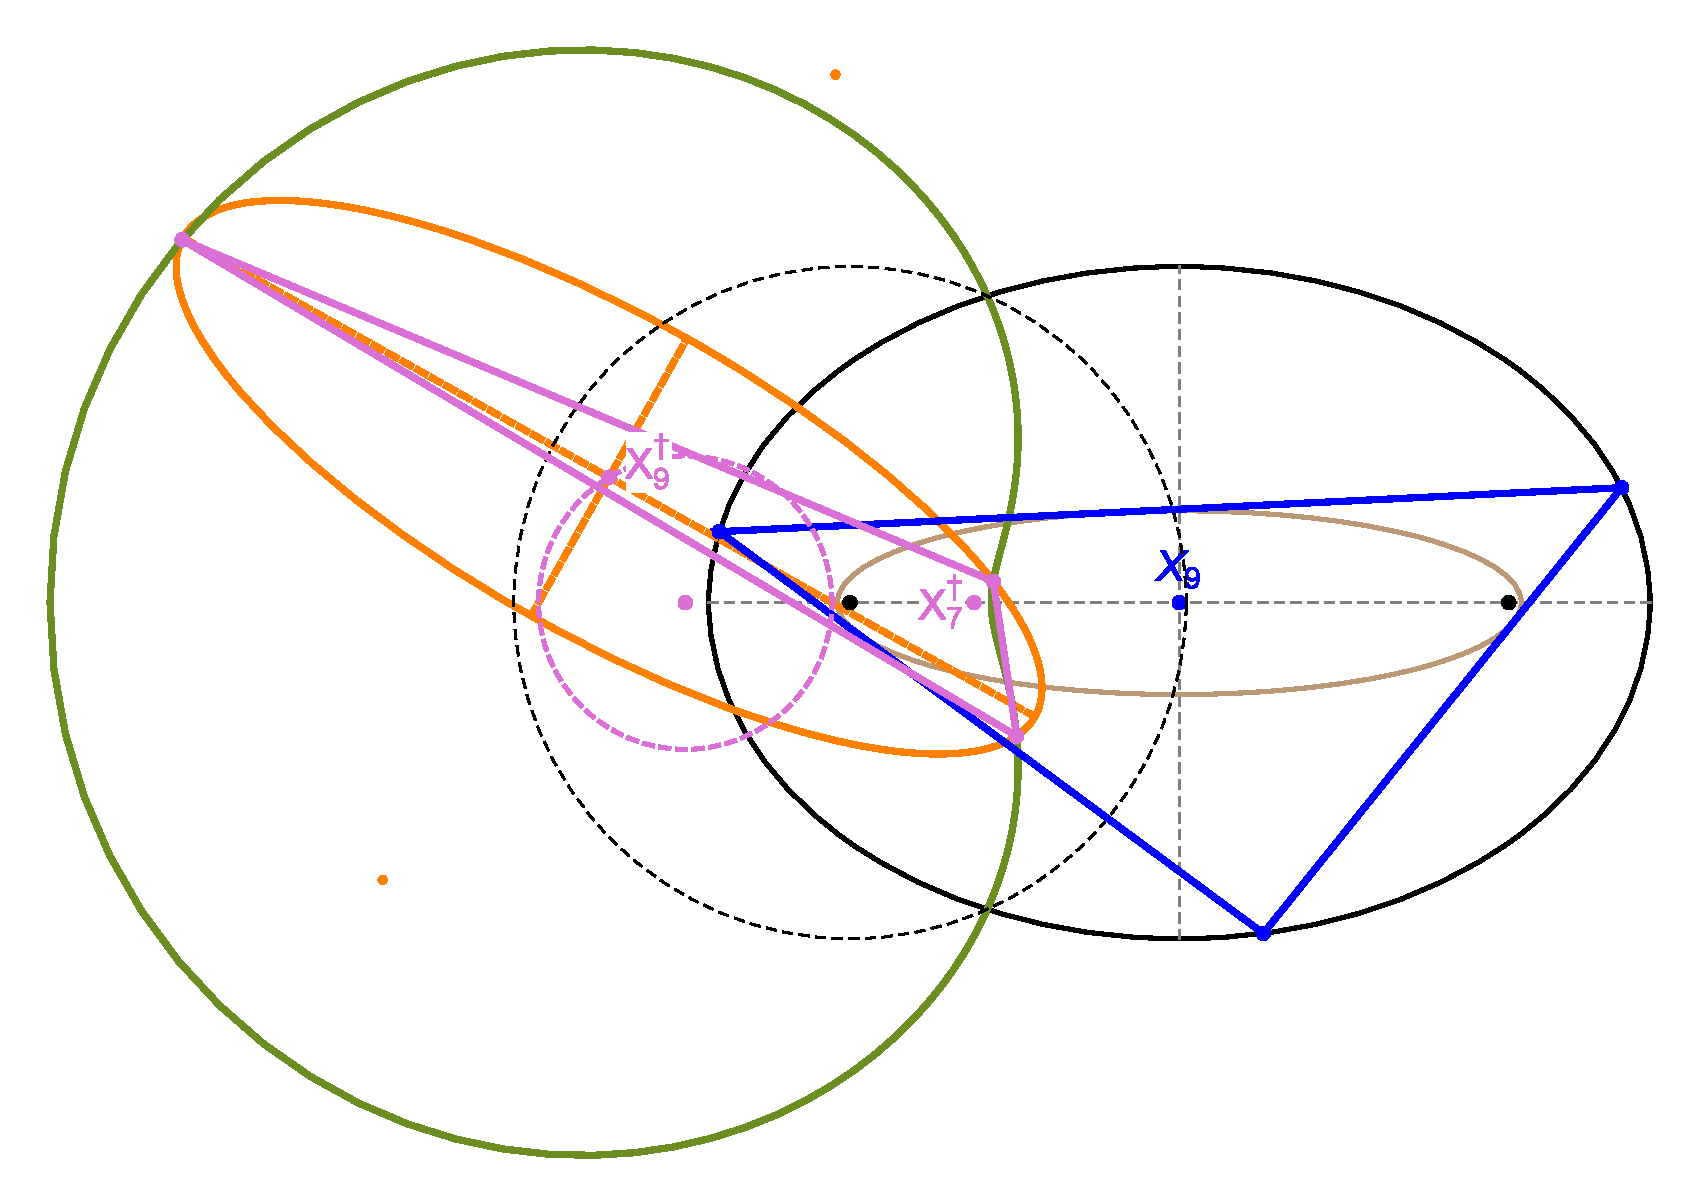
\includegraphics[width=\textwidth]{pics_08_030_n3_rotating_billiard.eps}
    \caption{The moving circumbilliard (orange) to focus-inversives (pink) rigidly translate and rotate (invariant semi-axes). Their center $X_9^\dagger$ sweeps a circle. The location of the stationary Gergonne point $X_7^\dagger$ is also shown. \href{https://youtu.be/LOJK5izTctI}{Video 1}, \href{https://youtu.be/Y-j5eXqKGQE}{Video 2}}
    \label{fig:08-n3-moving-billiard-table}
\end{figure}

\begin{proposition}
Over the 3-periodic family, the Mittenpunkt $X_9^\dagger$ of focus-inversive triangles moves along a circle with center and radius given by:
\begin{align*}
    C_9^\dagger=&\left[-c\left(1+\rho^2 \frac{1}{2b^2}\right), 0\right] \\
    R_9^\dagger=&\rho^2\, \frac{2a^2-b^2-\delta}{2 a b^2}
\end{align*}
\label{prop:08-x9}
\end{proposition}

\section{Invariant area product}

Let $A_1^\dagger$ (resp. $A_2^\dagger$) denote the area of the $f_1$- (resp. $f_2$) inversive triangle family. Referring to Figure~\ref{fig:08-inv-pedals}:

\begin{proposition}
For $N=3$, the area product $A_1^\dagger A_2^\dagger$ of the two focus-inversive triangles is given by:

\[ A_1^\dagger A_2^\dagger= \frac{\rho^8}{8 a^8 b^2}  \left[\left( {a}^{4}+2\,{a}^{2}{b}^{2}+4\,{b}^{4} \right)\delta +  \frac{3 a^{4} b^{2}}{2}+a^6+4\,{b}^{6} \right]
\]
\end{proposition}

\begin{figure}
    \centering
    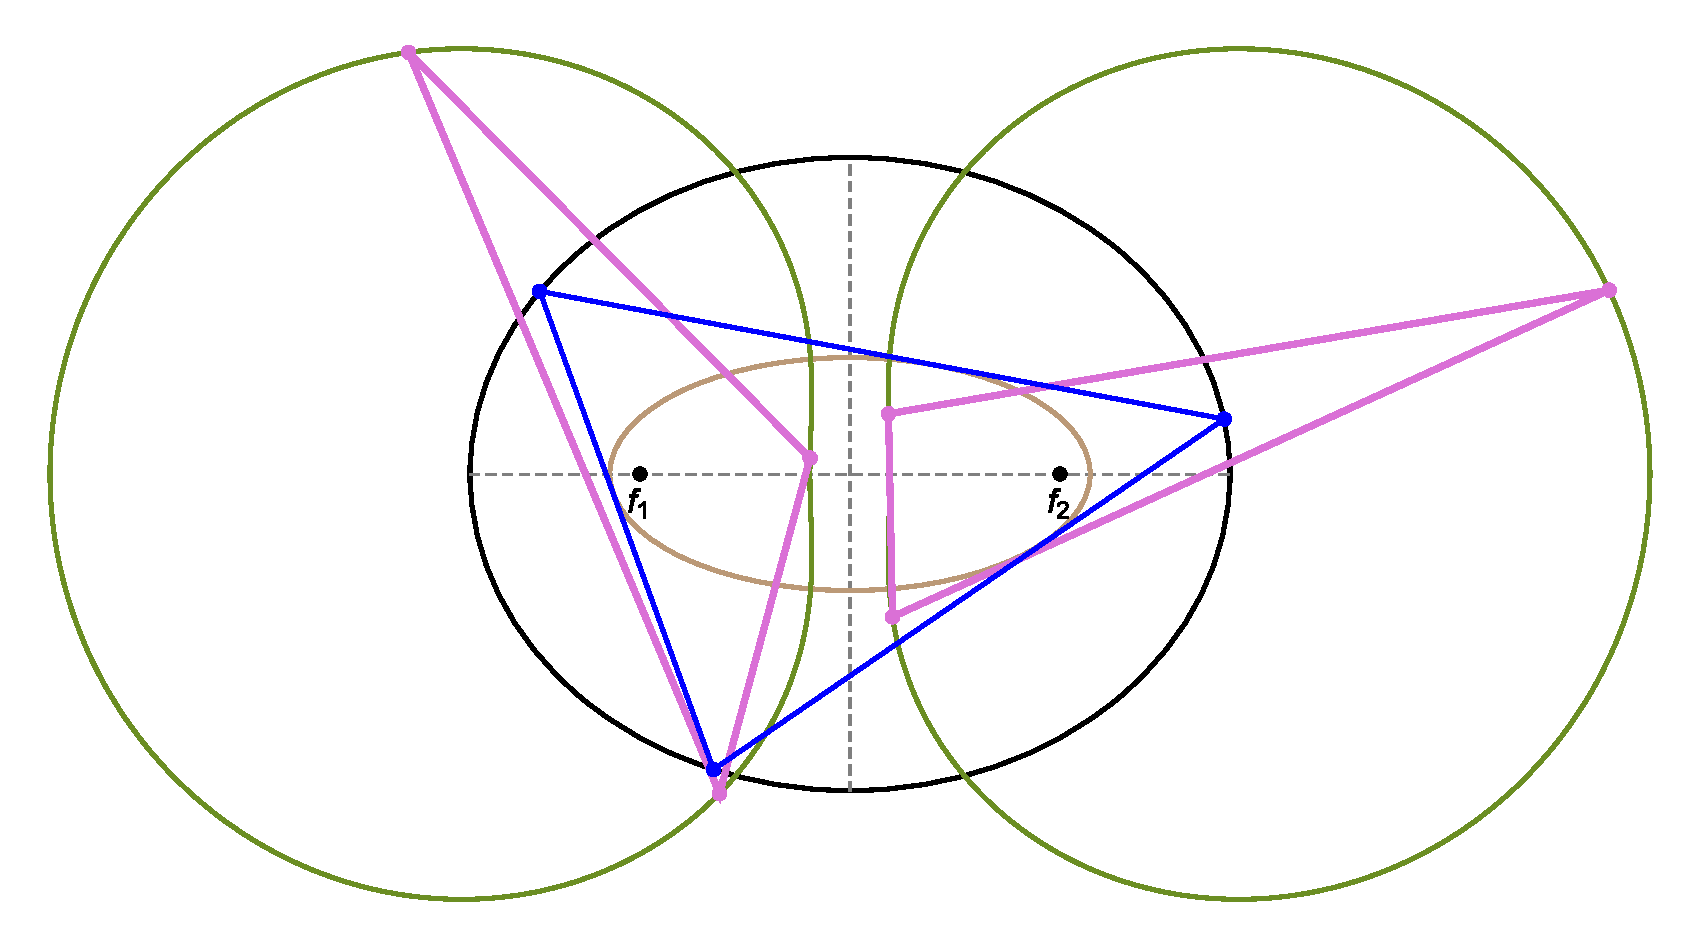
\includegraphics[width=\textwidth]{pics_08_040_n3_f1f2.eps}
    \caption{The area product of $f_1$- and $f_2$-inversive triangles (pink) is invariant. \href{https://youtu.be/0L2uMk2xyKk}{Video}, \href{https://bit.ly/3i1iPCM}{Live}}
    \label{fig:08-inv-pedals}
\end{figure}

\section{Circular loci galore!}

\begin{figure}
    \centering
    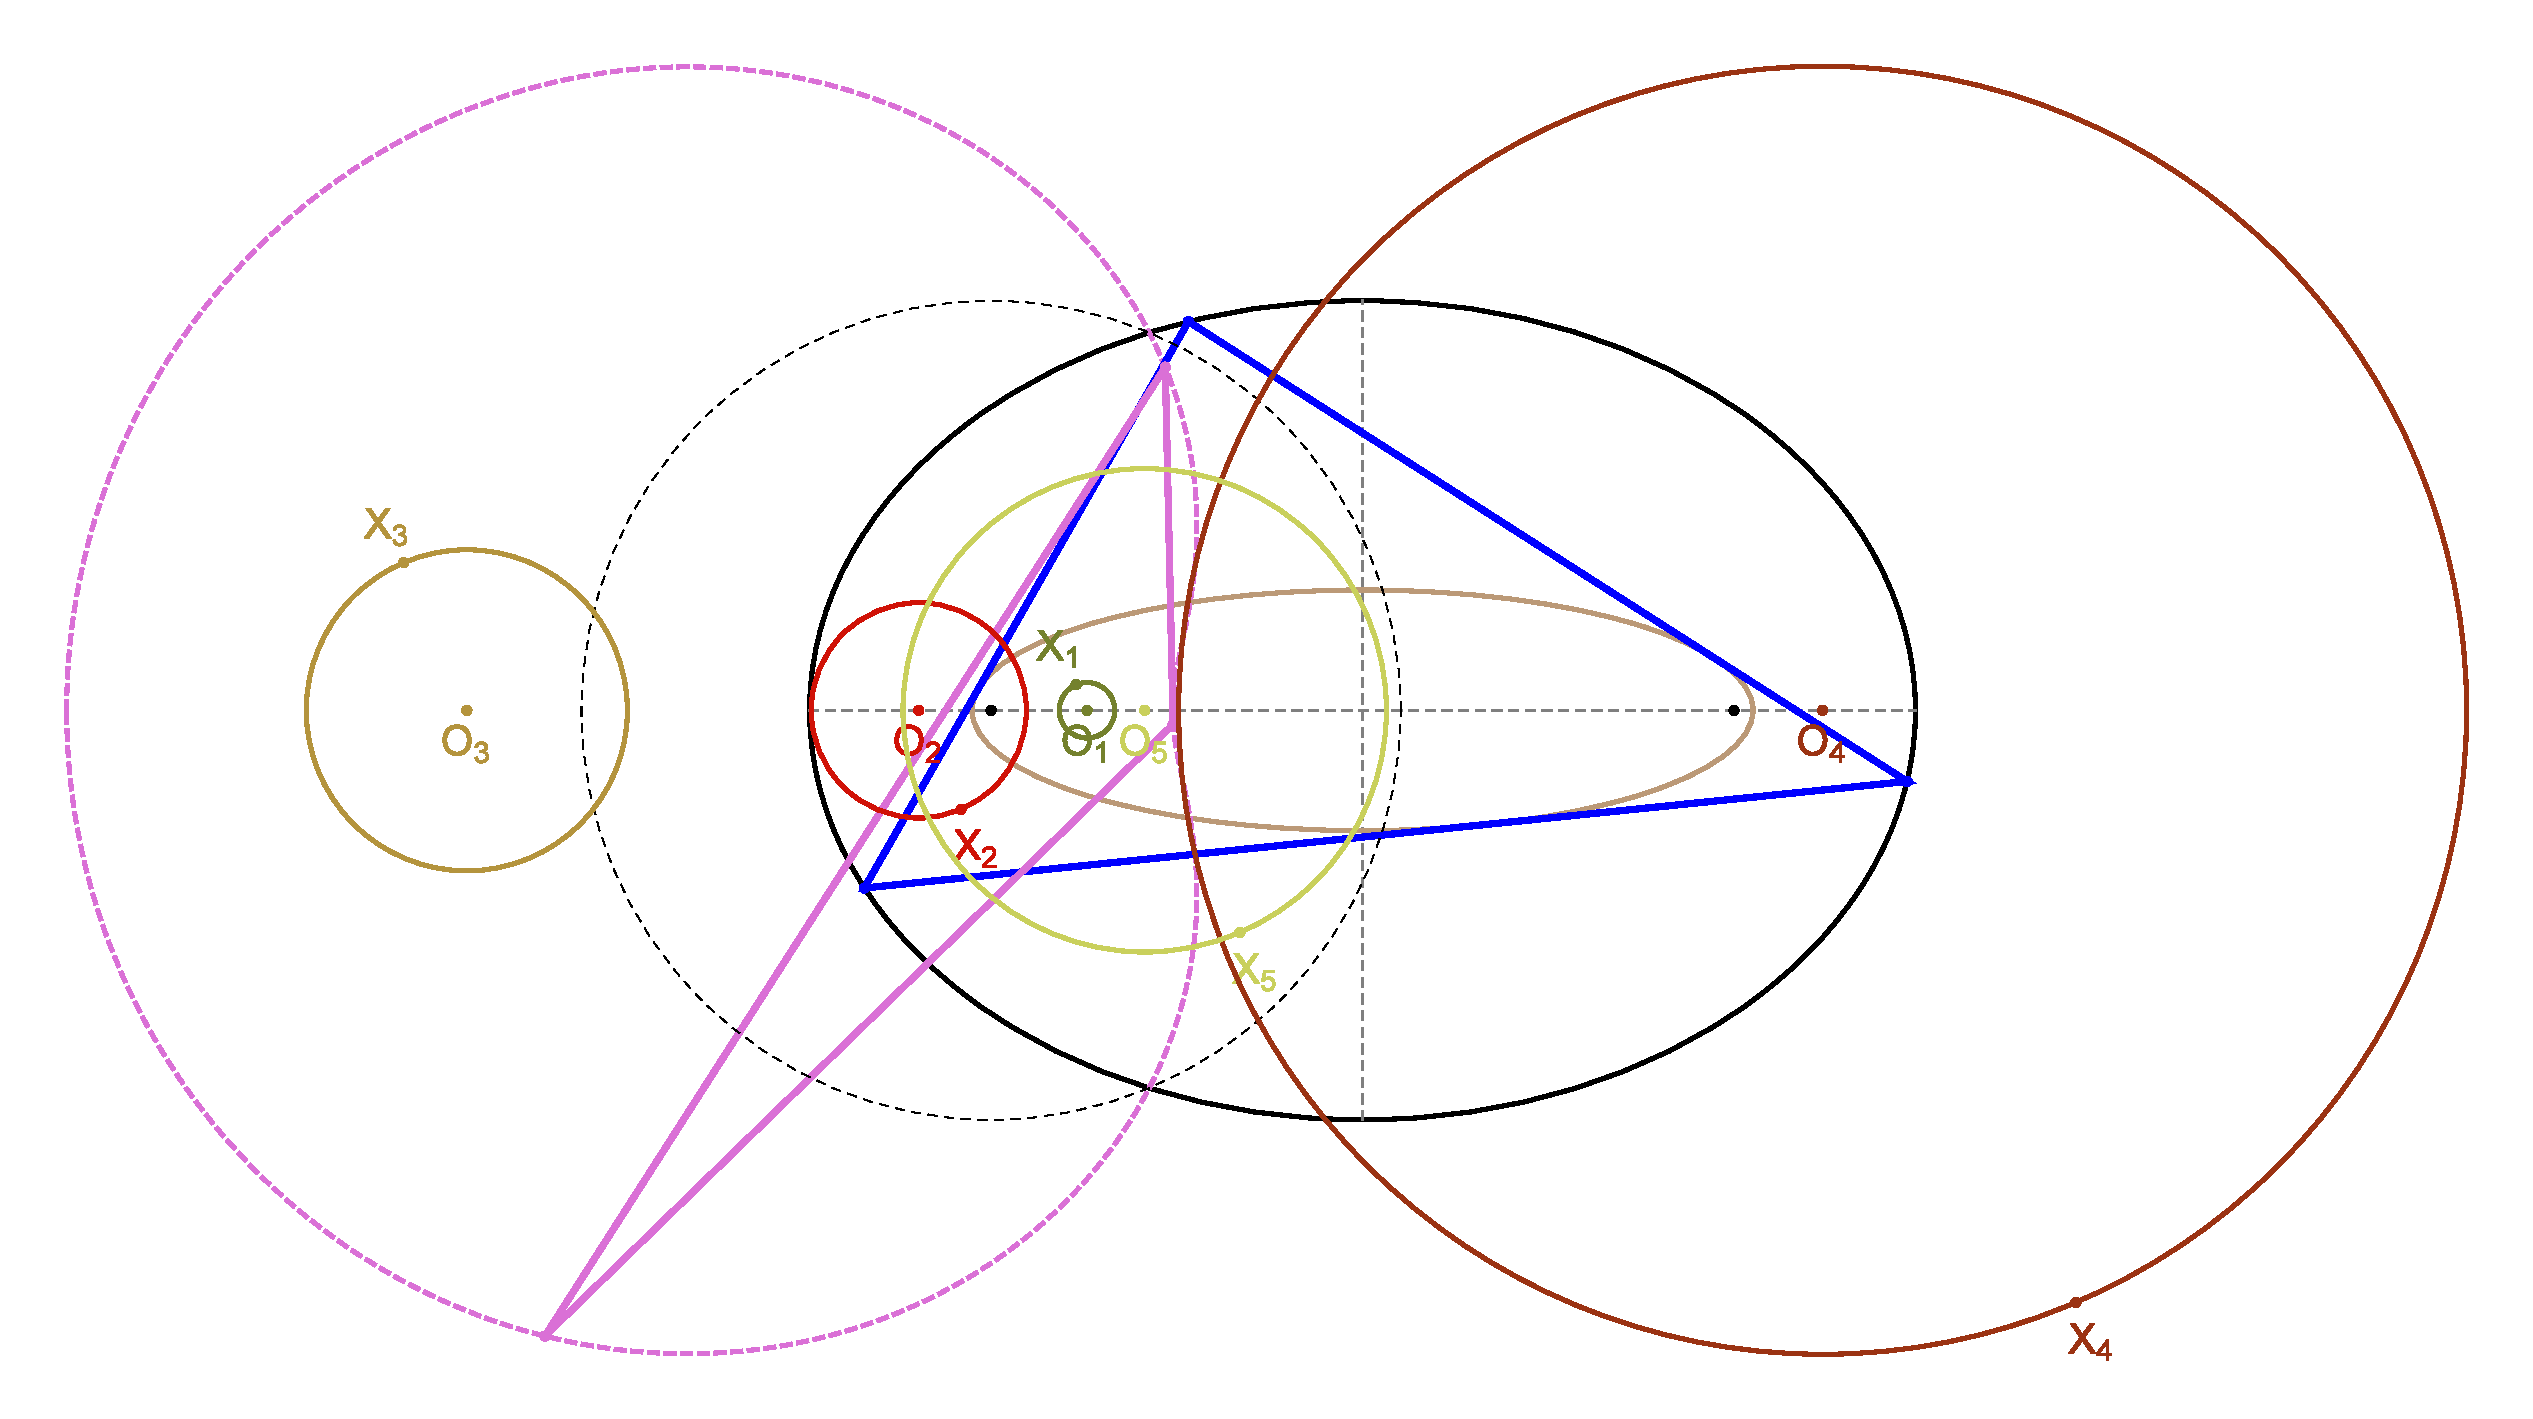
\includegraphics[width=\textwidth]{pics_08_050_n3_inv_loci12345}
    \caption{A focus-inversive 3-periodic (pink) is shown inscribed in Pascal's Limaçon (dashed pink). Also shown are the circular loci of $X_k^\dagger$, $k=1,2,3,4,5$ whose centers $O_i$ all lie on the billiard's major axis. \href{https://youtu.be/OAD2hpCRgCI}{Video}, \href{https://bit.ly/3fW3W1A}{Live}}
    \label{fig:08-n3-loci-12345}
\end{figure}

We saw above that the locus of $X_9^\dagger$ is a circle. A remarkable property of the focus-inversive family is its ability to produce circular loci of many triangle centers. Referring to Figure~\ref{fig:08-n3-loci-12345}, through CAS-assisted simplification we obtain:

\begin{proposition}
The locus of $X_1^\dagger$ is the circle given by:
\begin{align*}
C_1^\dagger=&\left[c\left(-1+\rho^2\frac{-2a^2+b^2+2\delta}{2b^4}\right), 0\right]\\
R_1^\dagger=&\rho^2\frac{-2\delta^2+b^4+(2a^2-b^2)\delta}{2ab^4}
\end{align*}
\end{proposition}

\begin{proposition}
The locus of $X_2^\dagger$ is the circle given by:

\begin{align*}
C_2^\dagger&=\left[-c\left(1+\rho^2\frac{2a^2-b^2-\delta}{3 a^2 b^2}\right),0\right]\\
R_2^\dagger&=\rho^2\frac{2 a^2-b^2-\delta}{3 a b^2}
\end{align*}
\end{proposition}

\begin{proposition}
The locus of $X_3^\dagger$ is the circle given by:
\begin{align*}
C_3^\dagger=&\left[-c\left(1+\rho^2\frac{a^2+b^2}{2b^4}\right), 0\right]\\
R_3^\dagger=&\rho^2\frac{a(-b^2+\delta)}{2b^4}
\end{align*}
\end{proposition}

\begin{proposition}
The locus of $X_4^\dagger$ is the circle given by:
\begin{align*}
C_4^\dagger=&\left[c\left(-1+\rho^2\frac{(b^2+\delta) \delta}{a^2 b^4}\right), 0\right]\\
R_4^\dagger=&\rho^2\frac{c^2(b^2+\delta)}{a b^4}
\end{align*}
\end{proposition}

\begin{proposition}
The locus of $X_5^\dagger$ is the circle given by:
\begin{align*}
C_5^\dagger=&\left[c\left(-1+ \rho^2\frac{a^4 - 3 a^2 b^2+2 b^4 + 2 b^2 \delta}{4 a^2 b^4}\right), 0\right]\\
R_5^\dagger=&\rho^2\frac{(3a^2-2b^2)b^2+(a^2-2b^2)\delta}{4a b^2}
\end{align*}
\end{proposition}

\begin{proposition}
The locus of $X_{100}^\dagger$ is the circle given by:

\begin{align*}
C_{100}^\dagger&=\left[-c\left(1+\rho^2\frac{1}{b^2}\right),0\right]\\
R_{100}^\dagger&=\rho^2\frac{a}{b^2}
\end{align*}
\end{proposition}

Note: The locus of $X_{11}^\dagger$ is also a circle, see \cref{exe:08-x11}.

\section{A rule for circular loci?}

Recall \cref{sec:06-loci-types} where 42 triangle centers are identified (from within the first 200 in \cite{etc}), whose loci over billiard 3-periodics are ellipses.

\begin{observation}
Amongst the first 200 triangle centers listed on \cite{etc}, the following triangle centers $X_k^\dagger$ sweep conics over the focus-inversive family:

\begin{itemize}
\item Circles (40): 1, 2, 3, 4, 5, 8, 9, 10, 11, 12, 20, 21, 35, 36, 40, 46, 55, 56, 57, 63, 65, 72, 78,  79, 80, 84, 90, 100, 104, 119, 140, 142, 144, 145, 149, \textbf{150}\footnote{See \cref{que:08-x150}.}, 153, 165, 191, 200.
\item Ellipses (4): 69, 75, 85, 86.
\end{itemize}
\end{observation}

Comparing these with the list in \cref{sec:06-loci-types} for the confocal family, one realizes that the only ones missing are $X_7$ (stationary over the inversive family) and the ``swans'' $X_k$, $k=$88, 162, and 190. i.e., triangle centers which by construction lie on the billiard, see \cref{fig:08-x88-x162}.

\begin{figure}
    \centering
    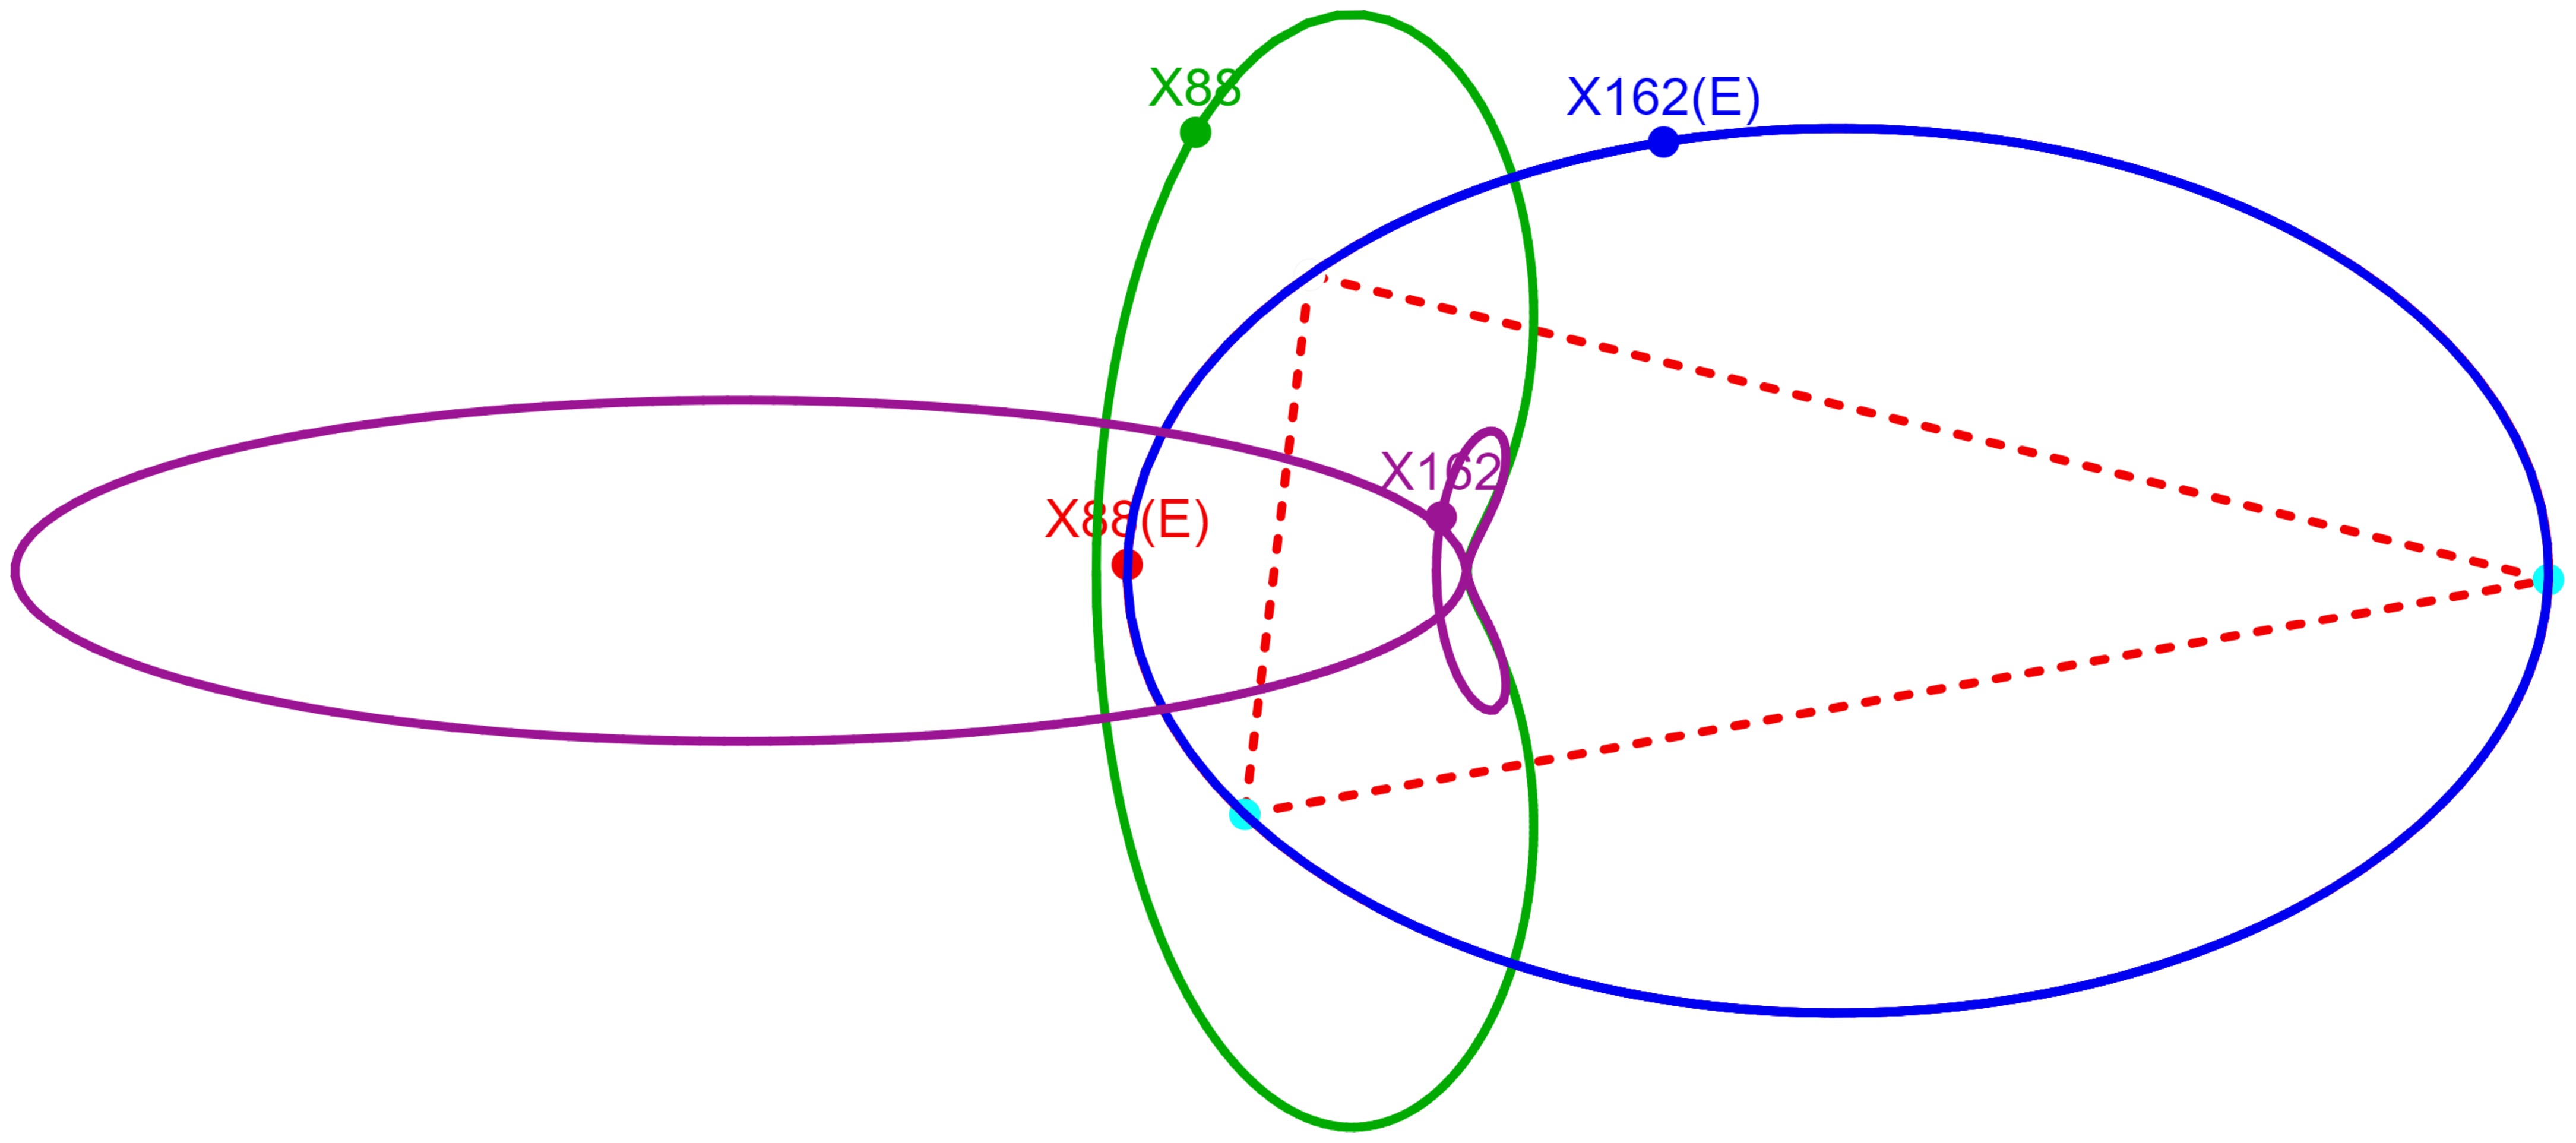
\includegraphics[width=\textwidth]{pics_08_070_x88_x162}
    \caption{Over billiard 3-periodics (dashed red) the loci of both $X_{88}$ and $X_{162}$  coincide with the billiard (blue). However, when taken as centers of the the focus-inversive triangles (not shown), their loci are clearly non-elliptic (green and purple). Live app: \href{https://bit.ly/32XfPyZ}{X88+X162}, \href{https://bit.ly/3lF3TsO}{X88+X100}}
    \label{fig:08-x88-x162}
\end{figure}

Experimentally, in the range $k{\leq}1000$, if the locus of $X_k$ is an ellipse over billiard 3-periodics (excluding the cases where the locus is the billiard itself), then the locus of $X_k^\dagger$ over the focus-inversive family is a circle. Therefore:

\begin{conjecture}
If the the locus of some triangle center $X$ is an ellipse over billiard 3-periodics, then the locus of $X^\dagger$ over the inversive family is a circle.
\end{conjecture}

The following cases do not invalidate the conjecture but are noteworthy:

\begin{itemize}
    \item Though $X_{100}$ is a swan, its focus-inversive locus is circular.
    \item Though $X_{658}$ is swan, its focus-inversive locus is an ellipse.
    \item Though the locus of $X_{150}$ is non-elliptic over billiard 3-periodics, that of $X_{150}^\dagger$ is a circle, see \cref{fig:08-x150}.
    \item Though the billiard locus of $X_{934}$ (blue) is a curve with two self-intersections, its focus-inversive locus is a circle, see it \href{https://bit.ly/3fUicrY}{Live}.
\end{itemize}

% still needs to test: 1156, 1492, 1821, 2349, 2580, 2581, 3257, 4598, 4599, 4604, 4606, 4607, 8052, 20332, 23707, 24624, 27834, 32680.

\begin{figure}
    \centering
    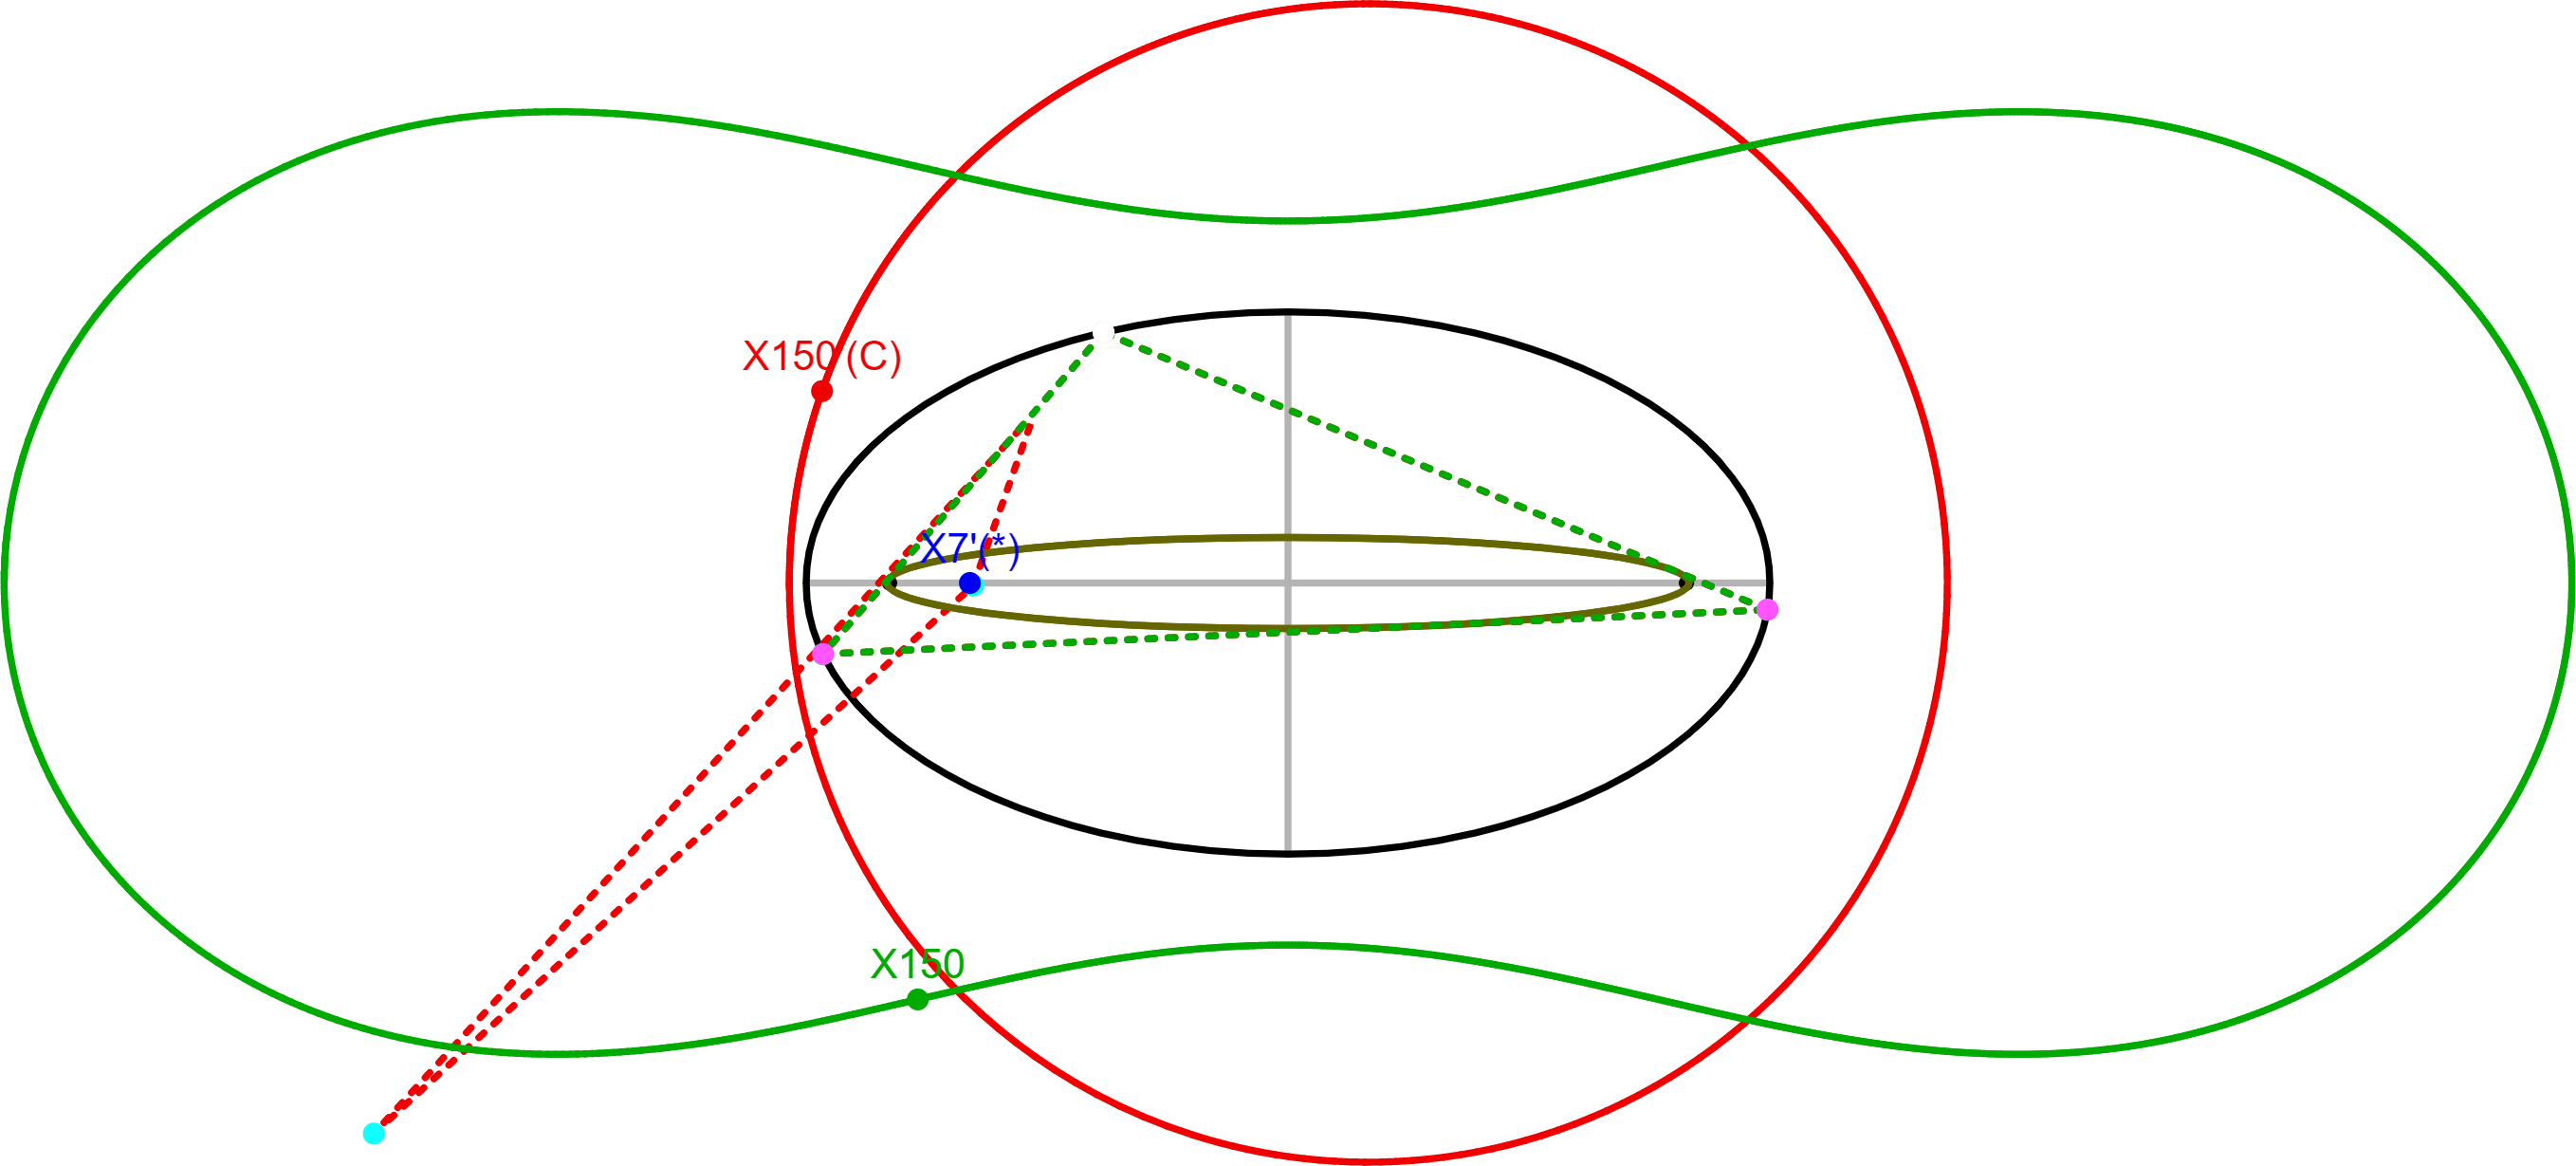
\includegraphics[width=\textwidth]{pics_08_060_x150.png}
    \caption{Though over billiard 3-periodics the locus of $X_{150}$ is non-elliptic, its locus over the focus-inversive family is a circle. \href{https://bit.ly/34v5Pgz}{Live}.}
    \label{fig:08-x150}
\end{figure}

\subsection{Centroidal loci: a tale of three circles}

Let $C_0$, $C_1$, $C_2$ denote the vertex, perimeter, and area centroids of polygon, respectively. In \cite[Thm 1]{schwartz2016-com} it was shown that the loci of $C_0,C_2$ over Poncelet families are ellipses, though this not hold in general for $C_1$.

For triangles, $C_0=C_2=X_2$ and $C_1=X_{10}$ \cite[Spieker Center]{mw}. Per above we already know that the loci of $X_{2}$ and $X_{10}$ over the focus-inversive family are circles. Therefore, and referring to Figure~\ref{fig:n3-centroids}:

\begin{corollary}
The loci of the $C_i^\dagger$, $i=1,2,3$ of the focus-inversive family are circles.
\end{corollary}

\begin{figure}
    \centering
    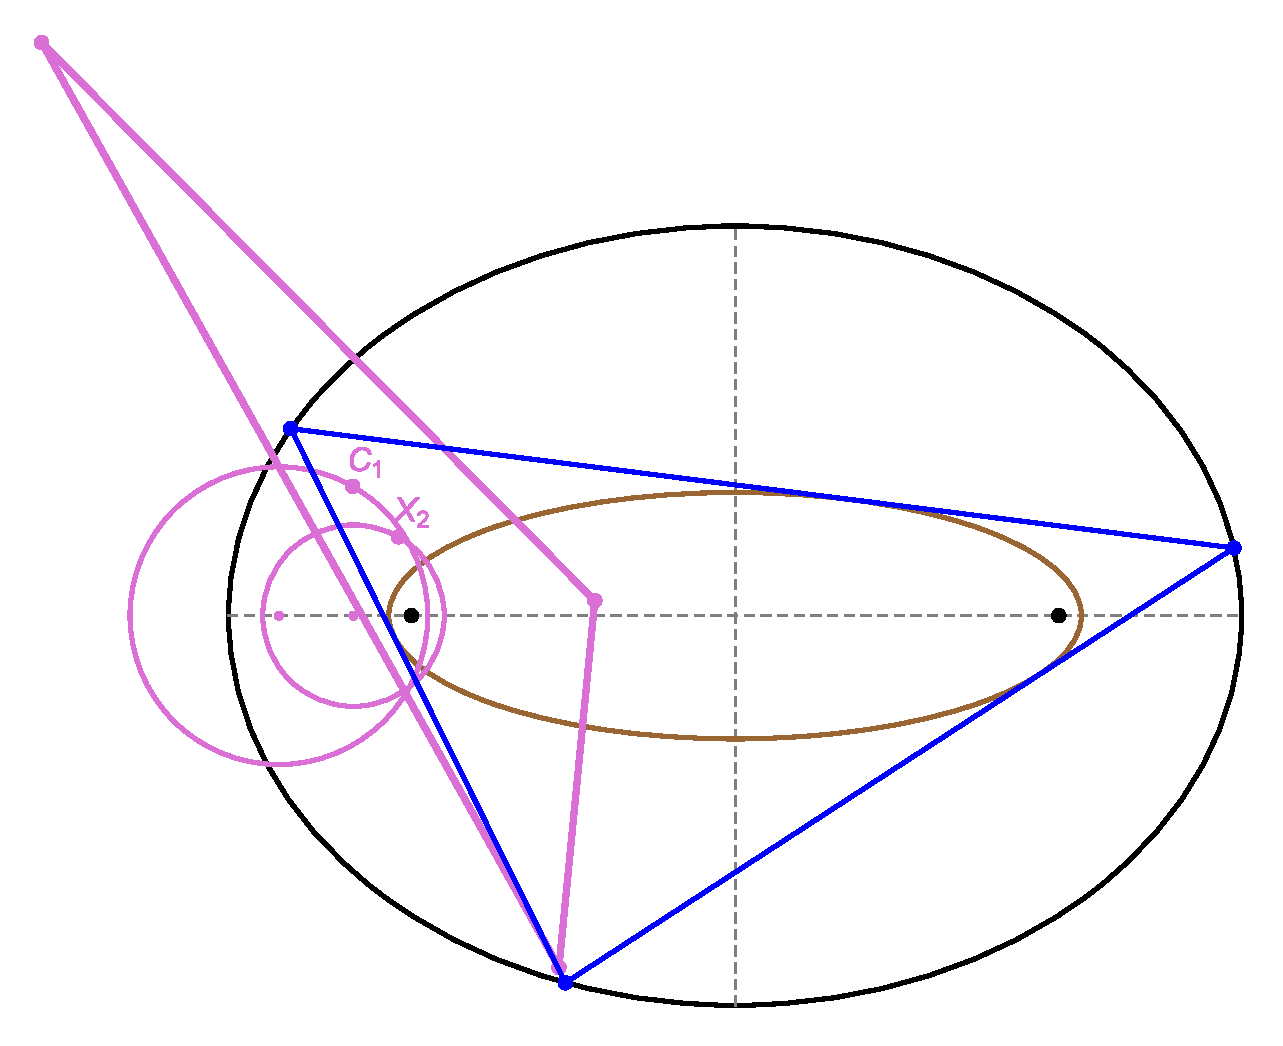
\includegraphics[width=.7\textwidth]{pics_08_080_n3_inv_centroids.eps}
    \caption{Circular locus of the focus-inversive $X_2$ and the perimeter centroid $C_1^\dagger=X_{10}^\dagger$. Note that for triangles, the former coincides with both the vertex and area centroids. \href{https://bit.ly/3kYnGlP}{App}}
    \label{fig:n3-centroids}
\end{figure}

\section{A focus-inversive doppelgänger}

\cref{cor:04-poristic-polar-image} in \cref{sec:04-poristic} states that the poristic family is the polar image of billiard 3-periodics with respect to a circle of radius $\rho$ centered on a focus. Let $R$ and $d$ denote the radius of the poristic circumcircle and $d=|X_3-X_1|$. If $a,b$ are the semi-axes of the outer ellipse in the confocal pre-image, then these can be expressed as:

\begin{proposition}
\begin{align*}
R =&(2a^4 - 2a^2b^2 + b^4 + (2a^2 -b^2)\delta  )a\rho^2/b^6\\
d=&(2a^2 - b^2 + 2\delta)c\rho^2a^2/b^6
\end{align*}
\end{proposition}

Recall every pair of circles is associated with two so-called {\em limiting points} $\ell_1$ and $\ell_2$ about which the inversion of the pair yields a new pair of concentric circles, see \cite[Limiting points]{mw}.

Let $\Cm$ and $\Cm'$ denote the incircle and circumcircle of the poristic family. Referring to \cref{fig:08-concentric-inverted}, it can be shown:

\begin{observation}
One of the limiting points -- call it $\ell_1$ -- of the bicentric circle pair coincides with a focus -- call it $f_1$ -- of its confocal polar pre-image. Furthermore, $\ell_1$ is internal to both circles.
\label{obs:08-ell1}
\end{observation}

\begin{figure}
    \centering
    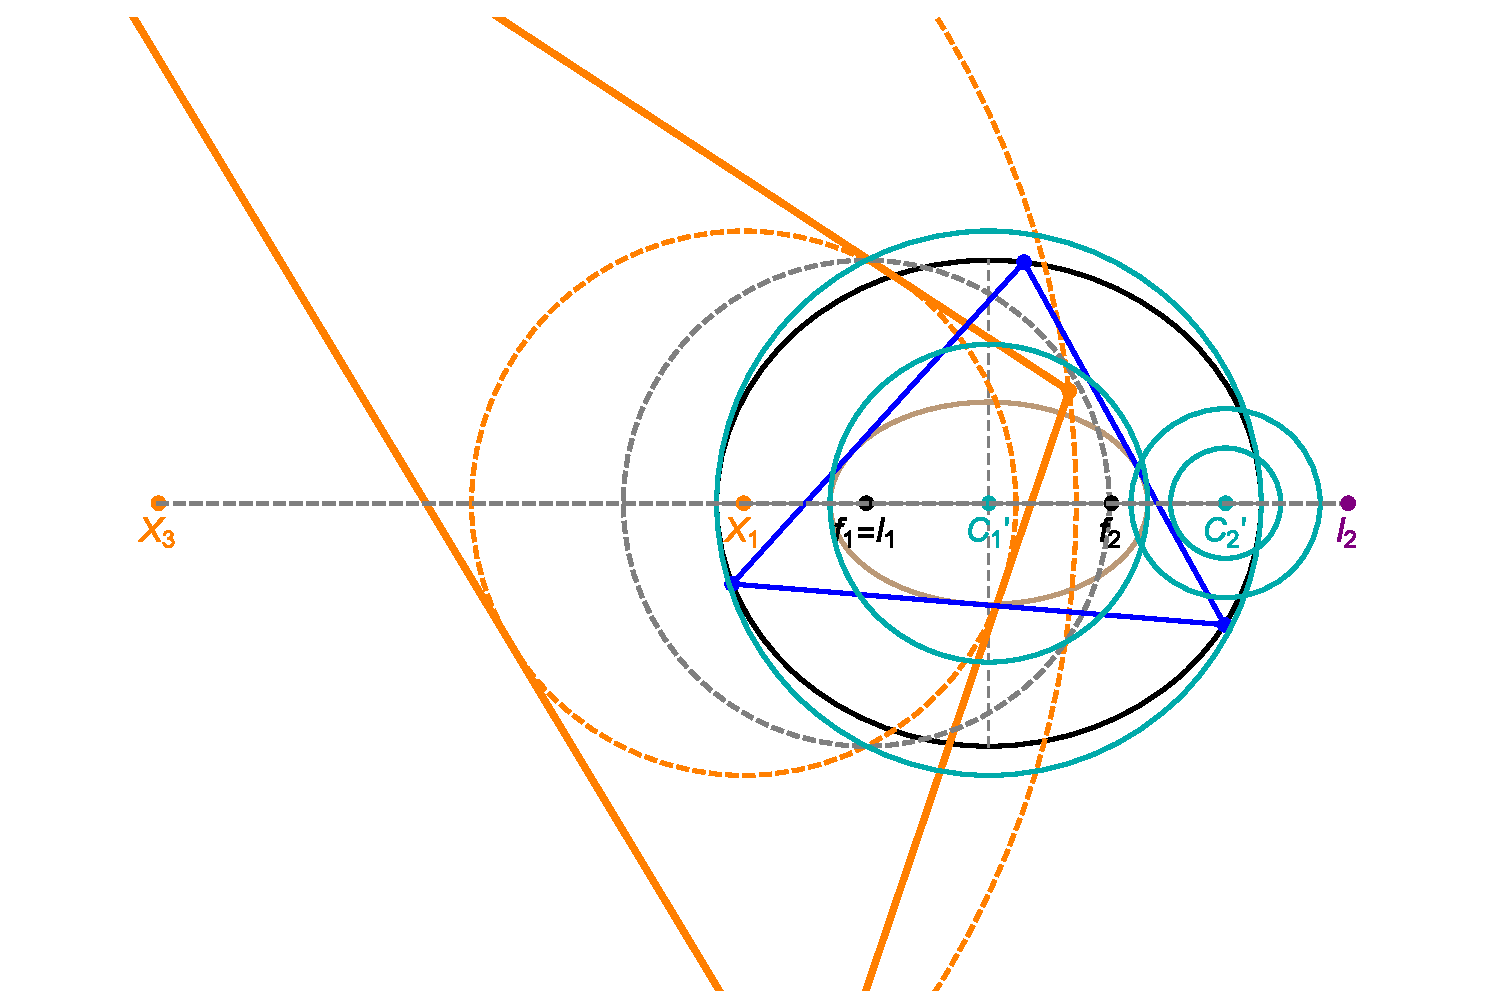
\includegraphics[width=\textwidth]{pics_08_100_concentric_inverted_pairs.eps}
    \caption{Billiard 3-periodic (blue) and its polar image (orange) with respect to a circle (dashed gray) centered on the left focus. Said polar family is poristic and interscribed between two circles $\Cm$ and $\Cm'$ (dashed orange) whose centers are labeled $X_3$ and $X_1$. Also shown are the two limiting points $\ell_1$ and $\ell_2$ of this pair of circles. Notice that $\ell_1$ (resp. $\ell_2$) is internal (resp. external) to $\Cm$ and $\Cm'$ and coincides with the billiard left focus (resp. lies to the right of the billiard center). Also shown are the two pairs of concentric circles (light blue) which are inversive images of $\Cm$ and $\Cm'$ about $\ell_1$ and $\ell_2$, respectively. Notice the circles in the first pair are tangent to the billiard (black) and confocal caustic (brown) at their major vertices, respectively.}
    \label{fig:08-concentric-inverted}
\end{figure}

Classic inversive geometry yields:

\begin{proposition}
Triangles of the focus-inversive family are identical to the pedal triangles of the poristic family with respect to $f_1=\ell_1$. 
\label{prop:08-focus-inversive-pedals}
\end{proposition}

\begin{figure}
    \centering
    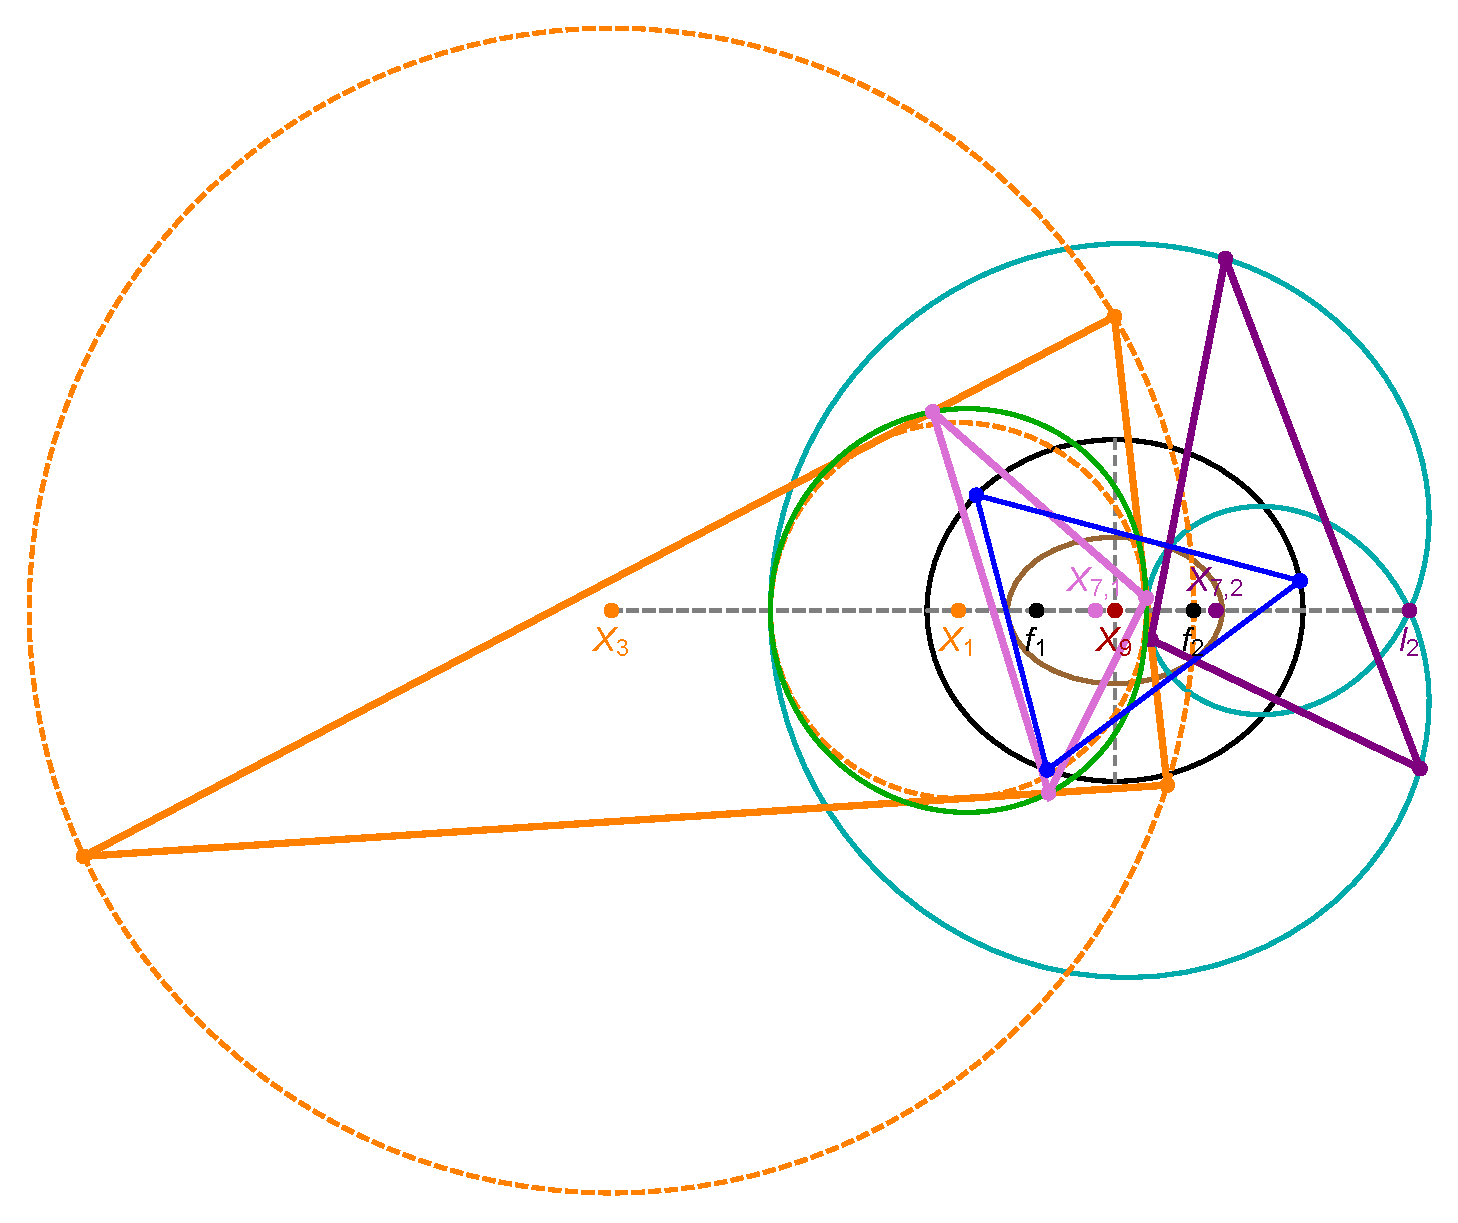
\includegraphics[width=.9\textwidth]{pics_08_090_n3_bicentric.pdf}
    \caption{A billiard 3-periodic (Blue), and its polar image with respect to the left focus, i.e., the poristic family (solid orange). The focus-inversive family (pink) has invariant perimeter and can also be regarded as the pedal triangle of the poristic family with respect to said focus. The latter coincides with the interior limit point of the poristic circle pair. A second  triangle (purple) is shown which is the pedal with respect to the (exterior) limiting point $\ell_2$ of the poristic circle pair. Its perimeter is also invariant. The Gergonne points $X_{7,1}$ and $X_{7,2}$ of either pedal family are stationary. \href{https://bit.ly/379HU8l}{live}}
    \label{fig:08-n3-bicentric-pedals}
\end{figure}

Let $L^{\dagger\dagger}$ denote the perimeter of the pedal triangle with respect to the non-focal limiting point $\ell_2$. Referring to \cref{fig:08-n3-bicentric-pedals}:

\begin{proposition}
Over the poristic family, 
 $L^{\dagger\dagger}$ is invariant and given by:

\[ L^{\dagger\dagger} = {\frac { \left( 9\,{R}^{2}-{d}^{2} \right)  \left( {R}^{2}-{d}^{2}
 \right) \sqrt {2}\rho^2}{16\,{R}^{4}d}\sqrt { \left( {R}^{2}-{d}^{2}
 \right) ^{{\frac{3}{2}}}\sqrt {9\,{R}^{2}-{d}^{2}}+ 3R^4 + 6R^2d^2 - d^4}}\]
\end{proposition}

\cref{eq:04-bic-cos} in  \cref{sec:04-poristic} provides an expression for the invariant sum of cosines of the poristic family in terms of the semi-axes $a',b'$ of its billiard polar pre-image. Interestingly:

\begin{proposition}
The sum of cosines of pedal triangles to the bicentric family with respect to either limiting point is invariant and identical to that of the poristic themselves.
\end{proposition}

Let $X_7^{\dagger\dagger}$ denote the Gergonne point of the pedal of bicentrics with respect to their (external) limiting point:

\begin{proposition}
$X_7^{\dagger\dagger}$ is stationary over the poristic family and given by:

\[X^{\dagger\dagger}=-\frac{(R^2  -d^2) ((R^2 - d^2)^{3/2}\sqrt{9R^2 - d^2} - 3R^4 - 6R^2d^2 + d^4)}{16d R^4}
\]
\end{proposition}


